\documentclass[10pt]{article}
\usepackage[a4paper,margin=1.6cm]{geometry}
\usepackage[T1]{fontenc}
\usepackage{lmodern}
\usepackage[utf8]{inputenc}
\usepackage[french]{babel}
\usepackage{amsmath,amssymb}
\usepackage{booktabs,tabularx,array}
\usepackage{graphicx}
\usepackage[detect-all]{siunitx}
\usepackage[font=small,labelfont=bf,labelsep=period,skip=3pt]{caption}
\frenchsetup{SmallCapsFigTabCaptions=false}
\addto\captionsfrench{\renewcommand{\tablename}{Tableau}}
\usepackage{tikz}
\usetikzlibrary{positioning,arrows.meta,fit}
\usepackage{microtype}

\sisetup{output-decimal-marker={,},group-separator={\,},group-digits=integer,group-minimum-digits=4,table-number-alignment=center}
\setlength{\parindent}{0pt}
\setlength{\parskip}{4pt}
\setlength{\tabcolsep}{4pt}
\setlength{\textfloatsep}{6pt plus 2pt}
\setlength{\floatsep}{6pt plus 2pt}
\setlength{\intextsep}{6pt plus 2pt}
\renewcommand{\arraystretch}{1.08}
\makeatletter
\renewcommand\section{\@startsection{section}{1}{0pt}{1.0ex plus .3ex}{0.5ex}{\normalfont\large\bfseries}}
\renewcommand\subsection{\@startsection{subsection}{2}{0pt}{0.8ex plus .2ex}{0.3ex}{\normalfont\normalsize\bfseries}}
\makeatother

\begin{document}

\begin{center}
{\Large\bfseries Sous-titrage automatique de journaux arabes en français}\\[2pt]
{\normalsize Cascade (S0), traduction directe de la parole (SeamlessM4T v2) et projecteur audio-texte (S3), évalués sur FLEURS et testés en direct}\\[4pt]
Sami Nakib, Fatima Aguel, Nicolas Wujczak, Paul Douat et Hanine Attia\\
{\small Rédaction : Paul Douat. CY Tech, cours de NLP, 23 octobre 2026}
\end{center}

\begin{abstract}
\noindent Nous comparons trois chaînes de sous-titrage français pour des journaux télévisés arabes : une cascade Whisper small puis Opus-MT (S0), le traducteur de la parole SeamlessM4T v2, et S3, qui relie un encodeur audio gelé à Qwen2.5-1.5B par un projecteur entraîné. S3 transcrit l'arabe de MGB-2 avec un WER de 14,26\,\% sur un test filtré. Comme MGB-2 n'a pas de français, la traduction est évaluée sur FLEURS (267 phrases, références humaines), où Seamless dépasse S0 de 11,2 points de chrF++. Sur le texte arabe, le traducteur spécialisé NLLB-1.3B obtient 31,3 BLEU, alors que Qwen2.5-1.5B affiné par LoRA passe seulement de 15,2 à 17,3. L'application Kalam, construite à partir de ces mesures, a sous-titré le direct d'Al Jazeera avec un retard moyen de 3,8\,s lors d'un essai de cinq minutes.
\end{abstract}

\section{Introduction}
L'arabe est parlé par plus de 400 millions de personnes, mais il reste relativement délaissé par les grands modèles de langage. Sa part dans les données d'entraînement est très inférieure à son nombre de locuteurs, et la diglossie complique la tâche : l'arabe standard des bulletins coexiste avec des dialectes, libanais ou égyptien par exemple, que l'on entend dès qu'un invité prend la parole. Les corpus qui associent de la parole arabe à une traduction sont rares, et MGB-2, le grand corpus de journaux télévisés arabes, ne contient aucune référence française. Nos propres mesures illustrent cet écart. Utilisé comme traducteur, Qwen2.5-1.5B-Instruct laisse 8\,\% de ses sorties en arabe et n'atteint que 15 BLEU sur FLEURS, alors qu'un traducteur spécialisé de taille voisine, NLLB-1.3B, en obtient 31.

Nous cherchons donc à produire, avec des modèles ouverts et un seul GPU T4, des sous-titres français utilisables pour des journaux arabes, y compris en direct. Pour cela, nous comparons trois chaînes : une cascade Whisper small puis Opus-MT (S0), le traducteur de la parole SeamlessM4T v2, et S3, une architecture où un projecteur entraîné relie un encodeur audio gelé à Qwen2.5-1.5B. Nous construisons une référence française à partir de FLEURS, nous analysons le comportement du LLM et l'effet d'un affinage LoRA, puis nous déployons le meilleur assemblage dans Kalam. Cette application reçoit un fichier audio ou vidéo, un lien ou le micro, rend des sous-titres horodatés (SRT, VTT) et a été testée sur le direct d'Al Jazeera.

Ce plan n'était pas celui du départ. L'idée initiale était d'affiner Whisper, voire d'entraîner un modèle de zéro, mais ni les données appariées ni le temps disponible ne le permettaient. Le projet s'est donc recentré sur une cascade dont le traducteur est un LLM, que l'on peut analyser et adapter par LoRA, et que nous comparons à la traduction directe de SeamlessM4T. Pour supprimer l'étape textuelle entre la reconnaissance et le LLM, nous avons ensuite proposé un projecteur audio vers LLM (S3), avec l'encodeur de Cohere plutôt que celui de Whisper, qui complète chaque entrée à 30\,s et perd ainsi environ deux tiers du calcul sur un segment de 10\,s. Comme MGB-2 n'a pas de français, FLEURS est devenu notre référence, et ses résultats ont fixé le choix final : Opus-MT, le plus rapide, pour le texte provisoire, et NLLB-1.3B, le plus fidèle, pour le texte définitif. La mise en conditions réelles sur le direct d'Al Jazeera a enfin révélé des défauts que les essais sur fichiers ne montraient pas, et que nous avons corrigés (section~\ref{sec:direct}).

\subsection{Cas d'usage}
Le premier public visé est celui des journalistes francophones au Liban et dans le monde arabe, qui suivent les chaînes d'information en direct et doivent repérer vite qui parle et de quoi. Les organisations humanitaires et les ONG ont des besoins voisins sur le terrain, lors d'entretiens, de réunions ou face aux médias locaux. Les enseignants et les chercheurs qui travaillent sur des sources arabes peuvent sous-titrer une archive vidéo et en exporter la transcription horodatée. Comme le texte arabe peut aussi être affiché, l'outil sert enfin à l'apprentissage de la langue, avec des sous-titres bilingues. Dans tous ces cas, le texte produit aide à suivre et à repérer une information, mais il doit être relu avant d'être cité ou publié.

\section{Données et systèmes}
\subsection{Corpus}
Pour l'apprentissage, nous disposons de MGB-2 (QCRI, défi SLT 2016) : environ 1\,200 heures d'Al Jazeera Arabic diffusées de 2005 à 2015, en arabe standard et dialectal, avec des transcriptions réalignées automatiquement dont l'écart à la parole est mesuré par le WMER. Après filtrage (5 à 25\,s, au moins six mots, WMER au plus 15\,\%, au plus 200 segments par émission), il reste 232\,227 segments (675,4\,h), répartis par émission grâce à un hachage MD5 pour qu'aucune émission du test ne serve à l'entraînement. Or MGB-2 ne contient aucune traduction française, et nous évaluons donc la traduction sur FLEURS, en appariant par identifiant le test \texttt{ar\_eg} au test \texttt{fr\_fr} : 267 phrases, 49,4 minutes de parole lue, chacune avec sa traduction humaine.

\subsection{Travail sur les données}
\label{sec:donnees}
La constitution des données a représenté une part importante du travail. Pour la traduction de texte, l'équipe a assemblé un corpus parallèle arabe-français à partir de quatre sources d'OPUS, GlobalVoices, News-Commentary, TED2020 et un échantillon de 20\,000 paires d'UNPC, soit 543\,237 paires en entrée. Un filtre de langue côté français, un rapport de longueur borné à $[0{,}6 ; 2{,}5]$ et un dédoublonnage exact en gardent 497\,658. Les membres arabophones de l'équipe ont relu un échantillon de 30 paires tiré avec une graine fixe : 27 sont correctes, 3 fausses ou désalignées, soit 10\,\% de paires erronées. Ils ont aussi aidé à traduire et à vérifier des traductions de l'arabe vers le français, jugé les cinq consignes de traduction essayées pour S3 sur cinq textes (la consigne retenue traduit les cinq sans introduction) et écrit les 8 phrases de journal de la grille de requêtes, conçues pour piéger les noms propres, les sigles, le dialecte libanais et les expressions idiomatiques. Pour les noms propres, un lexique de 396 entités a été extrait de Wikidata, chacune avec sa forme française et ses variantes d'écriture arabes. Côté parole, la sélection de MGB-2 décrite plus haut part de 354\,043 segments d'entraînement lus pour en retenir 232\,227, et l'appariement de FLEURS par identifiant de phrase fournit la référence française.

\subsection{Systèmes comparés}
S0 enchaîne un découpage par seuil d'énergie, Whisper small et Opus-MT, sans aucun entraînement. SeamlessM4T v2 large (2,3 milliards de paramètres) traduit directement la parole en texte français par fenêtres de 25\,s. S3 est notre architecture : l'encodeur de Cohere Transcribe (1\,895,3\,M de paramètres, gelé) produit des vecteurs de dimension 1\,280 à 12,5\,Hz, qu'un projecteur de 8,66\,M de paramètres (LayerNorm, 1280\,$\to$\,3072, GELU, 3072\,$\to$\,1536) place dans l'espace d'entrée de Qwen2.5-1.5B-Instruct, gelé lui aussi. Qwen transcrit l'arabe, puis un traducteur de texte produit le français. Seul le projecteur a été entraîné, sur 50\,000 segments (144,9\,h) et sur un Apple M5 Pro (AdamW, taux $10^{-3}$, lot effectif 16, bfloat16). Nous avons arrêté au pas 1\,730, soit 0,56 passage sur les deux prévus, et gardé le pas 1\,500, dont le WER de validation est de 13,4\,\% contre 159\,\% au pas 0. Sur 1\,000 segments de test tirés de 127 émissions inédites, S3 obtient un WER de 17,28\,\% et un CER de 9,66\,\%, puis 14,26\,\% et 7,22\,\% avec une limite de longueur et la suppression des répétitions. Toutefois, ces règles ont été réglées après avoir vu les boucles du test, si bien que ce dernier chiffre n'est pas une mesure aveugle. Le second temps prévu, la traduction directe depuis l'audio, n'a pas été réalisé : sans lui, Qwen recopie l'arabe dans 100\,\% des sorties quand on lui demande de traduire l'audio projeté.

Sur un journal de MGB-2 (émission 5331FFF2, 217 segments sans référence française), Seamless rend correctement François Hollande et Charlie Hebdo, mais traduit des «~incidents de tirs~» par «~accidents de tir~» et coupe une phrase sur «~depuis~», faute d'avoir la suite dans sa fenêtre de 25\,s. Dans S3, la reconnaissance confond les mots arabes signifiant «~décoration~» et «~augmentation~», et la traduction produit alors «~la quantité augmente~» : l'erreur du premier étage passe telle quelle dans le français.

\section{Évaluation sur FLEURS}
Les calculs ont tourné sur Kaggle (GPU T4, fp16) : BLEU et chrF++ avec sacreBLEU 2.6.0, COMET avec le modèle \texttt{wmt22-comet-da}, écarts testés par bootstrap apparié (300 tirages, graine 42, intervalle à 95\,\%). Le tableau~\ref{tab:systemes} compare les systèmes de bout en bout. Le tableau~\ref{tab:traducteurs} isole la traduction, chaque traducteur recevant la transcription arabe de référence.

\begin{table}[htbp]
\centering\small
\caption{Systèmes de la parole au français sur FLEURS \texttt{ar\_eg} (267 phrases, T4). RTF : temps de calcul rapporté à la durée audio, hors chargement.}
\label{tab:systemes}
\begin{tabular}{@{}l S[table-format=2.2] S[table-format=2.2] S[table-format=2.2] S[table-format=2.2] S[table-format=1.4] S[table-format=1.3] S[table-format=1.2]@{}}
\toprule
Système & {WER (\%)} & {CER (\%)} & {BLEU} & {chrF++} & {COMET} & {RTF} & {VRAM (Go)}\\
\midrule
S0 : Whisper small + Opus-MT & 46.41 & 24.04 & 11.81 & 35.04 & 0.5477 & \bfseries 0.088 & \bfseries 0.73\\
SeamlessM4T v2 large & \bfseries 8.58\rlap{$^a$} & 4.79\rlap{$^a$} & \bfseries 17.38 & \bfseries 46.22 & \bfseries 0.6901 & 0.146 & 3.48\\
Whisper-large-v3 (transcription seule) & 9.65 & \bfseries 3.41 & {n.a.} & {n.a.} & {n.a.} & 0.157 & 3.37\\
\bottomrule
\end{tabular}\\[2pt]
{\footnotesize $^a$ Transcription arabe de Seamless (langue cible arabe, RTF 0,113). n.a. : sans objet.}
\end{table}

\begin{table}[htbp]
\centering\small
\caption{Traduction de texte arabe vers français sur FLEURS (267 phrases). Latence médiane par phrase ; «~arabe~» : part des sorties restées en arabe.}
\label{tab:traducteurs}
\begin{tabular}{@{}l S[table-format=2.2] S[table-format=2.2] S[table-format=1.4] S[table-format=1.2] S[table-format=1.1] S[table-format=1.2]@{}}
\toprule
Traducteur & {BLEU} & {chrF++} & {COMET} & {Latence (s)} & {Arabe (\%)} & {VRAM (Go)}\\
\midrule
Opus-MT ar-fr & 24.31 & 49.58 & 0.7610 & \bfseries 0.19 & \bfseries 0 & \bfseries 0.17\\
NLLB-200 distillé 600M & 29.33 & 52.96 & 0.8065 & 0.46 & \bfseries 0 & 1.26\\
NLLB-200 distillé 1.3B & \bfseries 31.26 & \bfseries 55.19 & \bfseries 0.8261 & 0.82 & \bfseries 0 & 2.78\\
Qwen2.5-1.5B-Instruct & 15.23 & 40.24 & 0.7418 & 1.60 & 8.2 & 3.13\\
Qwen2.5-1.5B + LoRA (section~\ref{sec:lora}) & 17.33 & 42.05 & 0.7629 & 2.14 & \bfseries 0 & 3.13\\
Qwen2.5-7B-Instruct nf4, 150 phrases & 24.27 & 50.80 & 0.8013 & 2.27 & 0.7 & 6.03\\
\bottomrule
\end{tabular}
\end{table}

Seamless bat S0 sur toutes les mesures de qualité, et le bootstrap le confirme : +11,18 points de chrF++ (de +9,19 à +13,57), +5,57 points de BLEU (de +3,19 à +7,71) et 37,8 points de WER en moins. La faiblesse de S0 tient à sa reconnaissance, car Whisper small se trompe sur près d'un mot sur deux et Opus-MT ne peut pas rattraper ces erreurs. Whisper-large-v3 transcrit presque aussi bien que Seamless : l'écart de WER, 1,07 point, est significatif mais petit, et Whisper a le meilleur CER. Côté texte, NLLB-1.3B l'emporte sur les trois métriques, Opus-MT est le plus rapide, et Qwen2.5-1.5B recopie l'arabe dans 8,2\,\% des cas. Ainsi, le meilleur système de bout en bout (17,4 BLEU) reste loin du meilleur traducteur de texte (31,3). La reconnaissance et la segmentation coûtent donc plus de dix points. FLEURS a aussi ses biais : la parole y est lue, en arabe standard, sur des thèmes encyclopédiques, et nos empreintes ECAPA n'y trouvent que des voix féminines. Ces scores ne valent donc qu'en partie pour un journal télévisé.

\section{Analyse du LLM}
\label{sec:llm}
Nous avons ouvert le décodeur de S3 sur une phrase de journal, «~le ministère libanais de la Santé a annoncé hier que les cas de choléra dans le Nord étaient passés à 120~». Le tokeniseur BPE coupe ses 14 mots arabes en 28 tokens, dont trois pour les chiffres de 120, contre 33 tokens pour 23 mots français : l'arabe consomme environ 2 tokens par mot, le français 1,4. Le gabarit ChatML encadre la consigne système, le texte et l'instruction par des balises \verb+<|im_start|>+, et la génération commence après la balise de l'assistant, au terme de 87 tokens d'entrée. Au premier pas, la softmax sur 151\,936 logits place «~La~», «~L~» et «~Le~» en tête, et les dix premiers tokens couvrent 98,8\,\% de la masse (tableau~\ref{tab:llm}). Pourtant, le décodage glouton rend «~La ministre de la Santé libanaise a annoncé lundi\dots{}~» : le chiffre est juste, mais le ministère devient une ministre et hier devient lundi. Monter la température aplatit la distribution et ajoute d'autres fautes, «~syrienne~» à $T=0{,}7$ malgré un top-$k$ de 5, «~Haute-Garonne~» à $T=1{,}2$ avec un top-$p$ de 0,9. C'est pourquoi l'application décode en glouton. Changer la consigne système ne modifie qu'un mot (Sénat ou Parlement), alors qu'un exemple few-shot corrige un «~excédent budgétaire~» en «~déficit~», bien que l'exemple tiré d'OPUS soit hors sujet. En revanche, l'historique reste le point faible : avec deux phrases arabes précédentes, le modèle de base recopie l'arabe ou traduit le contexte au lieu de la phrase, défaut que le LoRA corrige et que nous avons retrouvé en direct. Sur notre grille de 24 requêtes (16 phrases FLEURS, 8 phrases de journal piégées par des noms propres, des sigles, du dialecte libanais et des expressions idiomatiques), le chrF++ moyen des phrases FLEURS passe de 37,89 à 41,54 avec le LoRA. Les chiffres y survivent, mais les deux modèles inventent le nom du ministre libanais de l'Énergie et ratent la FINUL.

\begin{table}[htbp]
\centering\small
\caption{Premier token généré par Qwen2.5-1.5B-Instruct : logits et probabilités (à gauche), effet de la température (à droite).}
\label{tab:llm}
\begin{tabular}{@{}l S[table-format=2.2] S[table-format=1.4] c l S[table-format=1.3] S[table-format=1.3] S[table-format=1.2]@{}}
\toprule
Token & {Logit} & {Probabilité} & \hspace{1.5em} & Température & {Top-1} & {Top-5} & {Entropie (nats)}\\
\midrule
La  & 22.30 & 0.5516 & & $T=0{,}2$ & 0.987 & 1.000 & 0.08\\
L   & 21.30 & 0.2029 & & $T=0{,}7$ & 0.674 & 0.998 & 0.90\\
Le  & 21.28 & 0.1998 & & $T=1{,}2$ & 0.478 & 0.930 & 1.70\\
\bottomrule
\end{tabular}
\end{table}

\section{Adaptation LoRA du traducteur}
\label{sec:lora}
Nous avons affiné Qwen2.5-1.5B-Instruct en traduction de texte avec un LoRA de rang 16 ($\alpha=32$, dropout 0,05) sur \texttt{q\_proj}, \texttt{k\_proj}, \texttt{v\_proj} et \texttt{o\_proj}, soit 4,36\,M de paramètres entraînables (0,28\,\%). Les 20\,500 paires d'entraînement et les 500 de validation viennent de notre corpus OPUS filtré (section~\ref{sec:donnees}), et 29\,\% d'entre elles portent les phrases précédentes comme contexte à ne pas traduire. Un passage de 1\,281 pas (taux $2\times10^{-4}$, lot 16, fp16) a pris 54,2 minutes sur une T4. La perte de validation, calculée sur les seuls tokens de la traduction, tombe de 1,71 à 1,41 dès le pas 100, puis à 1,35 au dernier pas (figure~\ref{fig:lora}) : le modèle apprend d'abord le format de réponse, puis progresse lentement.

\begin{figure}[htbp]
\begin{minipage}[c]{0.49\linewidth}
\centering
\IfFileExists{../resultats/kaggle/nlp-lora-traduction/courbe_perte.png}{%
  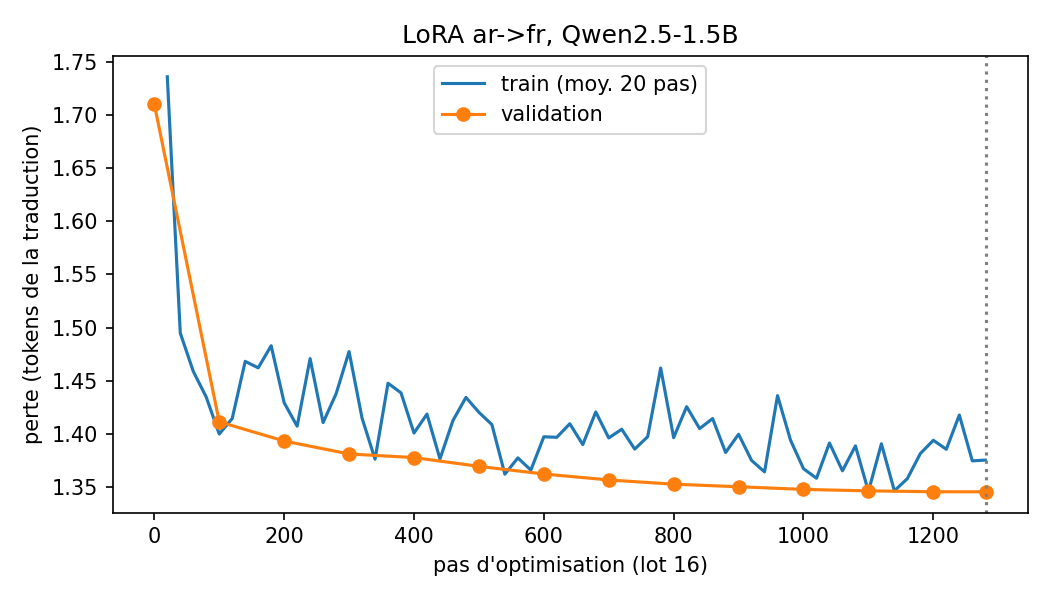
\includegraphics[width=\linewidth]{../resultats/kaggle/nlp-lora-traduction/courbe_perte.png}%
}{%
  \fbox{\parbox[c][3.5cm][c]{0.9\linewidth}{\centering\footnotesize Image absente :\\ \texttt{resultats/kaggle/nlp-lora-traduction/courbe\_perte.png}}}%
}
\captionof{figure}{Perte d'entraînement (moyenne sur 20 pas) et de validation du LoRA.}
\label{fig:lora}
\end{minipage}\hfill
\begin{minipage}[c]{0.48\linewidth}
\centering\footnotesize
\captionof{table}{Qwen2.5-1.5B avant et après LoRA. Cascade : chrF++ derrière trois transcriptions arabes de FLEURS.}
\label{tab:lora}
\begin{tabular}{@{}ll S[table-format=2.2] S[table-format=2.2]@{}}
\toprule
Jeu & Mesure & {Base} & {LoRA}\\
\midrule
FLEURS (267) & BLEU & 15.18 & \bfseries 17.20\\
 & chrF++ & 40.25 & \bfseries 41.98\\
 & COMET & 0.7417 & \bfseries 0.7637\\
 & Arabe (\%) & 8.2 & \bfseries 0.0\\
OPUS val. (200) & BLEU & 10.74 & \bfseries 13.19\\
\quad avec contexte & BLEU & 9.66 & \bfseries 13.21\\
\midrule
Cascade & Whisper small & \bfseries 30.96 & 30.49\\
 & Seamless (arabe) & 39.42 & \bfseries 40.58\\
 & Whisper-large-v3 & 39.02 & \bfseries 39.95\\
\bottomrule
\end{tabular}
\end{minipage}
\end{figure}

Seul, le traducteur progresse sur toutes les mesures (tableau~\ref{tab:lora}) et ne laisse plus aucune sortie en arabe. En revanche, le gain n'est plus significatif en cascade : derrière les trois transcriptions, l'intervalle bootstrap de l'écart de chrF++ contient zéro (de $-0{,}19$ à $+2{,}98$ derrière Seamless, par exemple). Surtout, à taille comparable, le traducteur spécialisé NLLB-1.3B reste loin devant, avec 31,3 BLEU et 0,826 de COMET contre 17,3 et 0,763 pour Qwen affiné, ce qui explique que Kalam traduise avec NLLB plutôt qu'avec Qwen.

\section{Produit et mode direct : Kalam}
\label{sec:direct}
L'application de Paul Douat (\texttt{speech\_app}) fournit le socle : une API FastAPI avec une interface Gradio, une image Docker, un registre qui charge les modèles à la demande et n'en garde qu'un groupe en mémoire, et un déploiement sur Colab (T4) derrière un tunnel Cloudflare. Kalam y ajoute le direct (figure~\ref{fig:archi}) : S3 transcrit chaque segment, Opus-MT affiche aussitôt un texte gris provisoire (0,19\,s par phrase) et NLLB-1.3B le remplace par le texte définitif (0,82\,s), deux traducteurs choisis d'après le tableau~\ref{tab:traducteurs}. En parallèle, des empreintes ECAPA (speechbrain) regroupées en ligne signalent les changements de locuteur, avec un seuil de similarité cosinus de 0,45 en direct et de 0,30 dans le rapport. Sur FLEURS, deux lectures d'une même voix ont en moyenne une similarité de 0,557, contre 0,266 entre voix différentes. En fin de session, un rapport rassemble la diarisation, une relecture ciblée par Qwen2.5-7B (nf4), un résumé et l'export SRT. Pour une vidéo déposée, une minute de journal demande 26\,s de calcul, et Piper peut lire les sous-titres à voix haute.

\begin{figure}[htbp]
\centering
\begin{tikzpicture}[font=\footnotesize, >={Stealth[length=1.8mm]},
  box/.style={draw, rounded corners=1.5pt, align=center, inner sep=2.5pt, minimum height=9.5mm, text width=#1},
  box/.default=2.7cm,
  gel/.style={box=#1, dashed},
  gel/.default=2.3cm,
  det/.style={font=\scriptsize},
  fl/.style={->, semithick}]
  % ligne 1 : capture et transcription
  \node[box=2.5cm] (client) at (1.35,0) {Navigateur\\ou téléphone\\{\scriptsize micro, lien, fichier}};
  \node[box] (api) at (4.55,0) {Serveur FastAPI\\{\scriptsize WebSocket, ffmpeg}};
  \node[gel] (enc) at (8.0,0) {Encodeur Cohere\\{\scriptsize gelé}};
  \node[box=2.3cm, fill=black!12] (proj) at (10.75,0) {Projecteur\\{\scriptsize entraîné, 8,66\,M param.}};
  \node[gel=2.5cm] (qwen) at (13.6,0) {Qwen2.5-1.5B\\{\scriptsize gelé}};
  \node[draw, dotted, fit=(enc)(proj)(qwen), inner sep=3pt, label={[font=\footnotesize, inner sep=1pt]above:S3 : transcription de l'arabe}] (s3) {};
  % ligne 2 : affichage, traduction, rapport
  \node[box=2.5cm] (aff) at (1.35,-2.0) {Affichage\\{\scriptsize double passe :\\gris puis définitif,\\locuteur}};
  \node[box] (ecapa) at (4.55,-2.0) {ECAPA\\{\scriptsize speechbrain\\changement de voix}};
  \node[box] (opus) at (8.2,-2.0) {Opus-MT\\{\scriptsize texte gris\\0,19\,s par phrase}};
  \node[box] (nllb) at (11.8,-2.0) {NLLB-1.3B\\{\scriptsize texte définitif\\0,82\,s par phrase}};
  \node[box=2.8cm] (rap) at (16.15,-2.0) {Rapport de fin\\{\scriptsize diarisation ECAPA,\\résumé ScaleDown (arabe), export SRT}};
  % flux
  \draw[fl] (client) -- (api);
  \draw[fl] (api) -- (s3.west |- api);
  \draw[fl] (enc) -- (proj);
  \draw[fl] (proj) -- (qwen);
  \draw[fl] (s3.east |- qwen) -| node[pos=0.75, right, det, align=left]{texte\\arabe} (rap.north);
  \fill (16.15,-0.95) circle (1.2pt);
  \draw[fl] (16.15,-0.95) -| (opus.north);
  \draw[fl] (11.8,-0.95) -- (nllb.north);
  \draw[fl] (api) -- (ecapa);
  \draw[fl] (ecapa) -- (aff);
  \draw[semithick] (opus.south) -- ++(0,-0.3) coordinate (o1);
  \draw[semithick] (nllb.south) |- (o1);
  \draw[fl] (o1) -| (aff.south);
\end{tikzpicture}
\caption{Architecture de Kalam. Tirets : modèles gelés ; fond gris : seul module entraîné de S3. Le texte gris d'Opus-MT s'affiche d'abord, puis NLLB-1.3B le remplace.}
\label{fig:archi}
\end{figure}

Le 23 octobre, nous avons branché Kalam sur le direct YouTube d'Al Jazeera, lu par yt-dlp sur le serveur (tableau~\ref{tab:direct}). Le premier essai traduisait le texte définitif avec Qwen2.5-1.5B et deux phrases de contexte. Aucune sortie n'est restée en arabe, mais le petit modèle mêlait le contexte à la phrase : le texte gris, juste, «~Nétanyahou, qui veut gagner les élections\dots{}~», a été remplacé par «~Le projet américain-israélien\dots{}~», faux. Dans l'enregistrement de cet essai, «~président du syndicat des journalistes iraniens~» devient même «~Président des États-Unis~», juste après une phrase sur le Parti républicain américain. Nous avons coupé le contexte, ce qui a mis au jour un bug de Python, \texttt{l[-0:]} renvoyant toute la liste au lieu d'une liste vide. Le direct a révélé deux autres défauts, dont l'option \texttt{-re} de ffmpeg : prévue pour lire un fichier à la vitesse réelle, elle freinait un flux HLS déjà en direct, avec 18 phrases en 13 minutes contre environ 8 par minute sans elle (56 en 8,5 minutes). Quand le GPU saturait, le retard moyen montait à 5,0\,s. Le serveur saute désormais la passe grise lorsqu'il prend du retard, puis réutilise la dernière transcription à la clôture d'un segment. L'essai final avec NLLB a ensuite donné 23 phrases sans arabe et 3 voix repérées. Enfin, le rapport de fin prenait 773\,s pour 60 segments au premier essai, contre 61\,s pour 10 minutes d'audio après optimisation. Comme son résumé local recopiait les erreurs de traduction («~le Golfeur~», «~25 soldats~»), nous résumons maintenant le texte arabe de S3 par l'API ScaleDown, en 2,9\,s au lieu d'environ 110\,s, et les 17 horodatages cités renvoient tous à des segments réels.

\begin{table}[htbp]
\centering\small
\caption{Retard d'affichage du texte définitif sur le direct d'Al Jazeera (Colab, T4). n.m. : non mesuré.}
\label{tab:direct}
\begin{tabular}{@{}l S[table-format=2.0] S[table-format=1.2] S[table-format=1.1] S[table-format=2.2]@{}}
\toprule
Configuration & {Phrases} & {Retard moyen (s)} & {Médian (s)} & {p95 (s)}\\
\midrule
S3, Opus-MT, Qwen2.5-1.5B avec 2 phrases de contexte & 36 & 3.97 & {n.m.} & 6.67\\
S3, Opus-MT, NLLB-1.3B (essai final) & 23 & \bfseries 3.8 & \bfseries 2.9 & 6.7\\
Session où le GPU saturait & 60 & 5.0 & {n.m.} & 10.6\\
\bottomrule
\end{tabular}
\end{table}

\section{Limites et suite à donner}
L'évaluation gagnerait à être élargie. Un jeu de test plus vaste, tiré de journaux télévisés récents et accompagné d'une notation humaine, mesurerait mieux la fidélité sur les noms propres et les chiffres que des métriques automatiques calculées sur de la parole lue. Il permettrait aussi de comparer d'autres modèles de reconnaissance et de traduction dans des conditions identiques, notamment la chaîne complète S3 suivie de NLLB. Un GPU plus puissant que la T4 ouvrirait d'autres pistes : prolonger l'entraînement du projecteur au-delà de 0,56 passage, essayer des décodeurs plus grands et réduire le retard du direct. La validation de S3, tirée du jeu d'entraînement, et le seuil de locuteurs, calibré sur des voix féminines, seraient à reprendre sur des données plus variées. Le produit a par ailleurs des limites d'usage.

Kalam ne traduit que dans un sens, de l'arabe vers le français. Une conversation dans les deux sens, lors d'un entretien sur le terrain par exemple, demanderait le sens inverse, du français vers l'arabe, avec sa propre évaluation. La lecture vocale repose sur Piper, avec une voix générique que nous n'avons pas entraînée. Les dialectes restent par ailleurs hors du domaine d'entraînement : MGB-2 en contient une partie, mais FLEURS n'en a pas, et sur notre phrase piège en libanais les deux modèles rendent «~depuis le matin~» par «~dans l'après-midi~» ou «~à l'aube~».

Nos résultats invitent surtout à explorer des modèles très spécialisés, qui ne sont pas forcément des LLM. À taille comparable, le traducteur seq2seq NLLB-1.3B dépasse de près de 14 points de BLEU un LLM généraliste, même affiné par LoRA, et le projecteur de S3, avec 8,7\,M de paramètres, suffit à rebrancher un encodeur audio sur un décodeur gelé. La suite consiste donc à distiller ou à affiner un traducteur spécialisé sur des journaux arabes, puis à terminer le temps 2 de S3 pour traduire directement depuis l'audio. Il faudra en parallèle constituer une référence française sur des journaux télévisés récents, en commençant par les 217 segments déjà extraits de MGB-2, et conduire une évaluation humaine, d'abord sur la grille de 24 requêtes.

\section{Contributions et licences}
Sami Nakib a assuré la coordination, la préparation des données, les mesures, le mode direct, l'intégration et l'évaluation finale. Nicolas Wujczak a construit le temps 1 de S3, de l'encodage Cohere à l'entraînement du projecteur et à la transcription. Fatima Aguel a conduit les benchmarks de Seamless et de la traduction de texte, Hanine Attia la comparaison entre EmbeddingGemma et COMETKiwi. Paul Douat a écrit l'application \texttt{speech\_app} et rédigé ce rapport.

MGB-2, SeamlessM4T et NLLB-200 sont réservés à la recherche non commerciale, et les données de MGB-2 ne sont pas versionnées. La police ABC Areal de l'interface n'est pas redistribuée. Les extraits d'Al Jazeera servent à un usage académique, mais le résumé passe par un service externe (ScaleDown). Comme les sous-titres peuvent contenir des noms faux (section~\ref{sec:llm}), ils ne doivent pas être diffusés sans relecture.

\section*{Références}
{\footnotesize Ali et al., \emph{The MGB-2 Challenge}, SLT 2016. Conneau et al., \emph{FLEURS}, 2022. Meta, \emph{Seamless}, 2023. NLLB Team, \emph{No Language Left Behind}, 2022. Hu et al., \emph{LoRA}, 2021. Rei et al., \emph{COMET-22}, WMT 2022. Post, \emph{A Call for Clarity in Reporting BLEU Scores}, WMT 2018. Desplanques et al., \emph{ECAPA-TDNN}, Interspeech 2020. Résultats bruts : \texttt{resultats/kaggle/} et \texttt{resultats/direct/} du dépôt.\par}

\end{document}
